\chapter{Технологический раздел}


\section{Средства реализации}
\hspace{0.6cm}Для реализации программы были следующие языки программирования:
\begin{itemize}
	\item Python (v.3.9\cite{web:python}) для написания интерфейса программы и отрисовки рук. Python является простым в использовании средством для выполнения небольших задач, таких как чтение и запись, отрисовка оконного интерфейса;
	\item Prolog (SWI-Prolog\cite{web:prolog}) для написания функций проверки точек на корректность.
\end{itemize}

\section{Сборка и запуск проекта}
\hspace{0.6cm}Для сборки проекта используется встроенная система сборки языка Python.
 

\section{Описание структуры базы знаний}
\hspace{0.6cm}Каждый палец (кроме большого) определяется 4 точками (3 точки для большого), следовательно необходимо проверять 3 различных угла при сгибе пальцев (2 для большого), а также угол отклонения пальца при отведении пальца. Таким образом, каждому пальцу соответствует 4 типа проверок.
\begin{lstlisting}[caption=Знания о типах проверок каждого пальца, label=list:finger_check]
%finger_motion_type(FingerType, AbductionType, Flexion1, Flexion2, Flexion3).

finger_motion_type(thumb, bpprived, bppsgib1, bppsgib2, bppsgib2).
finger_motion_type(index, oprived, o2sgib1, o2sgib2, o2sgib3).
finger_motion_type(middle, oprived, o3sgib1, o3sgib2, o3sgib3).
finger_motion_type(ring, oprived, o4sgib1, o4sgib2, o4sgib3).
finger_motion_type(little, oprived, o5sgib1, o5sgib2, o5sgib3).
\end{lstlisting}
Каждому из типу проверок соответствуют диапазоны углов, которые допустимые при том или ином движении пальца.
\begin{lstlisting}[caption=Знания об амплитудах углов, label=list:angle_limits]
%angle_type_limits(Finger, MinAngle, MaxAngle)

angle_type_limits(bpabc, -80, 80).
angle_type_limits(bpbcd, -50, 50).
angle_type_limits(bpcde, -90, 90).
angle_type_limits(oabc, -80, 80).
angle_type_limits(obcd, -100, 100).
angle_type_limits(ocde, -90, 90).
angle_type_limits(between, -30, 30).

angle_type_limits(bpprived, -50, 50).
angle_type_limits(oprived, -60, 60).
angle_type_limits(bppsgib1, -50, 50).
angle_type_limits(bppsgib2, -100, 80).

angle_type_limits(o2sgib1, -120, 90).
angle_type_limits(o2sgib2, -100, 100).
angle_type_limits(o2sgib3, -100, 100).

angle_type_limits(o3sgib1, -120, 90).
angle_type_limits(o3sgib2, -100, 100).
angle_type_limits(o3sgib3, -80, 80).

angle_type_limits(o4sgib1, -120, 90).
angle_type_limits(o4sgib2, -100, 100).
angle_type_limits(o4sgib3, -80, 80).

angle_type_limits(o5sgib1, -120, 90).
angle_type_limits(o5sgib2, -100, 100).
angle_type_limits(o5sgib3, -80, 80).

angle_type_limits(bppz, -100, 100).
\end{lstlisting}
Также каждый из типов проверок отвечает за конкретную ось пространства, по которой проводится проверка.
\begin{lstlisting}[caption=Знания об осях типов проверок, label=list:angle_det_type]
%angle_det_type(Type, Axis)

angle_det_type(bpabc, all).
angle_det_type(bpbcd, all).
angle_det_type(bpcde, all).
angle_det_type(oabc, all).
angle_det_type(obcd, all).
angle_det_type(ocde, all).
angle_det_type(between, all).

angle_det_type(bpprived, x).
angle_det_type(oprived, x).
angle_det_type(bppsgib1, y).
angle_det_type(bppsgib2, y).

angle_det_type(o2sgib1, x).
angle_det_type(o2sgib2, x).
angle_det_type(o2sgib3, x).

angle_det_type(o3sgib1, x).
angle_det_type(o3sgib2, x).
angle_det_type(o3sgib3, x).

angle_det_type(o4sgib1, x).
angle_det_type(o4sgib2, x).
angle_det_type(o4sgib3, x).

angle_det_type(o5sgib1, x).
angle_det_type(o5sgib2, x).
angle_det_type(o5sgib3, x).

angle_det_type(bppz, z).
\end{lstlisting}
Попадание угла в диапазон определяется процедурой, которая для этого использует знание о рассматриваемом виде соединения (который устанавливается исходя из знания о рассматриваемом пальце).
\begin{lstlisting}[caption=Проверка попадания угла в диапазон, label=list:valid_angle]
%valid_angle - check if angle is valid for finger
valid_angle(Type, Angle):-
	angle_type_limits(Type, MinAngle, MaxAngle),
	MinAngle =< Angle, Angle =< MaxAngle.
\end{lstlisting}
Программой на Prolog для описания руки используются структуры Рука, Палец и Точка.
\begin{lstlisting}[caption=Структуры, label=list:structures]
point(X, Y, Z).

hand(
	finger(little, P0, P1, P2, P3),		%5|finger V
	finger(ring, P4, P5, P6, P7),		%4|finger IV
	finger(middle, P8, P9, P10, P11),	%3|finger III
	finger(index, P12, P13, P14, P15),	%2|finger II
	finger(thumb, P16, P17, P18),		%1|finger I
	P19, P20							
).	
\end{lstlisting}
Каждой структуре соответствует своя процедура проверки корректности точек.
\begin{lstlisting}[caption=Процедура проверки корректности точек руки, label=list:validate_hand]
validate_hand(hand:hand(Finger5, Finger4, Finger3, Finger2, Finger1, P19, Wrist)):-
	validate_finger(Finger5, P19, Wrist),
	validate_finger(Finger4, P19, Wrist),
	validate_finger(Finger3, P19, Wrist),
	validate_finger(Finger2, P19, Wrist),
	validate_finger(Finger1, P19, Wrist).
\end{lstlisting}
Процедура проверки корректности точек пальца состоит из двух правил: одно для большого пальца, второе - для остальных пальцев.
\begin{lstlisting}[caption=Процедура проверки корректности точек пальца, label=list:validate_finger]
validate_finger(finger(thumb, P1, P2, P3), P19, Wrist):-
	finger_motion_type(thumb, Abduction, Flex1, Flex2, _),
	validate_points(bpabc, P1, P2, P3),
	validate_points(Abduction, P3, P2, Wrist),
	validate_points(Flex1, P1, P2, P3),
	validate_points(Flex2, P1, P2, Wrist),
	validate_points(bppz, P1, P2, P3).
	
validate_finger(finger(Finger, P1, P2, P3, P4), P19, Wrist):-
	not(Finger == thumb),
	finger_motion_type(Finger, Abduction, Flex1, Flex2, Flex3),
	validate_points(oabc, P1, P2, P3),
	validate_points(obcd, P2, P3, P4),
	validate_points(Abduction, P4, P2, Wrist),
	validate_points(Flex1, P2, P1, P3),
	validate_points(Flex2, P4, P2, P3),
	validate_points(Flex3, P4, P3, Wrist),
	validate_points(bppz, P1, P2, P3).
\end{lstlisting}

\begin{lstlisting}[caption=Процедура проверки угла между точками на корректность, label=list:validate_angle]
validate_angle(Type, Point1, Point2, Point3) :-
	hand:angle_det_type(Type, Axis),
	get_angle(Axis, Point1, Point2, Point3, Angle),
	write_files:write_angle(Type, Angle),
	hand:valid_angle(Type, Angle).
\end{lstlisting}

\section{Взаимодействие с Python}
\hspace{0.6cm}Взаимодействие Prolog с Python осуществляется с помощью библиотеки PySwip. С помощью метода prolog.query(statement), куда мы передаем все параметры, вызывается основная процедура проверки всех точек. Для получения этих параметров мы читаем точки из текстового файла. После этого вызванная процедура начинает проверку допустимости рук. Если некоторые точки не образуют допустимый угол, то мы записываем эти точки в текстовой файл. Если руки образуют допустимое положение, то решением будет Result=<<Ok>>, если нет - Result=<<Not>>.

\begin{lstlisting}[caption=Основная процедура проверки корректности точек, label=list:validate_all]
validate_all(Working_Dir, Result,
	Point1, Point2, Point3, Point4, Point5, Point6, Point7,
	Point8, Point9, Point10, Point11, Point12, Point13, Point14,
	Point15, Point16, Point17, Point18, Point19, Point20, Point21,
	Point22, Point23, Point24, Point25, Point26, Point27, Point28,
	Point29, Point30, Point31, Point32, Point33, Point34, Point35,
	Point36, Point37, Point38, Point39, Point40, Point41, Point42
) :-
	working_directory(_, Working_Dir),
	open('points.txt', write, Stream),
	open('angles.txt', write, Stream2),
	close(Stream2),
	close(Stream),
	(  
		(
		validate_hand(
			hand:hand(
				finger(little, Point1, Point2, Point3, Point4),
				finger(ring, Point5, Point6, Point7, Point8),
				finger(middle, Point9, Point10, Point11, Point12),
				finger(index, Point13, Point14, Point15, Point16),
				finger(thumb, Point17, Point18, Point19),
				Point20, Point21
			)
		),
		validate_hand(
			hand:hand(
				finger(little, Point37, Point38, Point39, Point40),
				finger(ring, Point33, Point34, Point35, Point36),
				finger(middle, Point29, Point30, Point31, Point32),
				finger(index, Point25, Point26, Point27, Point28),
				finger(thumb, Point22, Point23, Point24),
				Point41, Point42
			)
		)
	)-> Result = "Ok"; Result = "Not"
).

\end{lstlisting}

\newpage

\section{Отрисовка руки}
\hspace{0.6cm}Отрисовка руки написана на языке Python с помощью библиотек Tkinter и OpenGL. Точки загружаются из текстового файла, которых должно быть 42. После проверки допустимости каркас рук выводится на экран. При этом если ребра окрашены красным цветом, то это означает, что положение отдельной части руки в этих трех точках недопустимо. Левая рука окрашена зелёным цветом, а правая - рыжим. Точки обозначены чёрными квадратами.
\hspace{0.6cm}Перемещать камеру возможно с помощью стрелок на клавиатуре, масштабирование осуществляется с помощью кнопок '+' и '-'.

\begin{figure}[ht!]
	\centering
	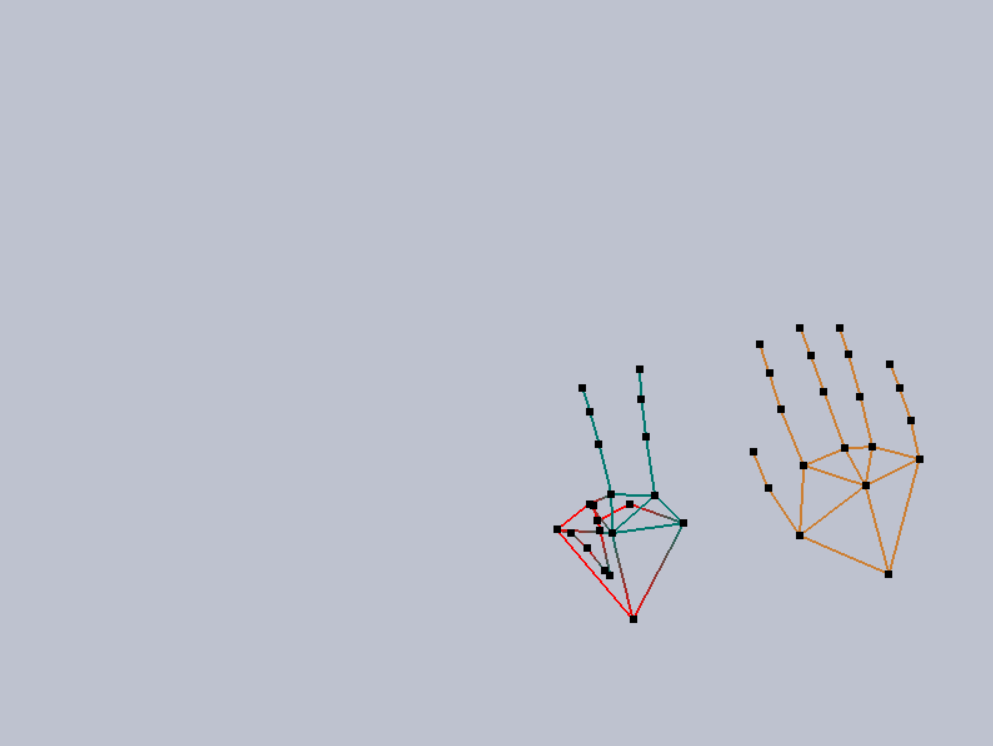
\includegraphics[scale=0.65]{example.png}
	\caption{Пример работы программы}
	\label{fig:example}
\end{figure}

